 \documentclass[tikz]{standalone}
% \usetikzlibrary{chains,shapes}

\usetikzlibrary{fit,arrows.meta}


\tikzset{
  value/.style={draw=black, font=\ttfamily},
  value label/.style={font=\ttfamily},
  next/.style={circle, fill=black},
  next label/.style={font=\ttfamily},
  node label/.style={draw=black, prefix after command= {\pgfextra{\tikzset{every label/.style={font=\ttfamily}}}}},
  link/.style={arrows={-Latex}},
  HEAD/.style={font=\ttfamily},
  NULL/.style={font=\ttfamily},
  PTR/.style={font=\ttfamily}
}


\tikzset{
  pics/llnode/.style args={#1/#2}{
    code = {
      \node[value] at (0,0) (#1 value) {#2};
      \node[value label] at (0,0.5) (#1 value label) {value\strut};
      \node[next] at (1.25,0) (#1 next) {};
      \node[next label] at (1.25,0.5) (#1 next label) {next\strut};

      \node[node label,fit={(#1 value) (#1 value label) (#1 next) (#1 next label)},label=#1] (#1) {};
    }
  },
  pics/llnodelabel/.style args={#1/#2/#3}{
    code = {
      \node[value] at (0,0) (#1 value) {#2};
      \node[value label] at (0,0.5) (#1 value label) {value\strut};
      \node[next] at (1.25,0) (#1 next) {};
      \node[next label] at (1.25,0.5) (#1 next label) {next\strut};

      \node[node label,fit={(#1 value) (#1 value label) (#1 next) (#1 next label)},label={[text=orange]#3}] (#1) {};
    }
  }
}


\begin{document}

% https://stackoverflow.com/questions/69377554/latex-nodes-with-text-do-not-align-vertically
% use strut to guarantee vertical alignment of text

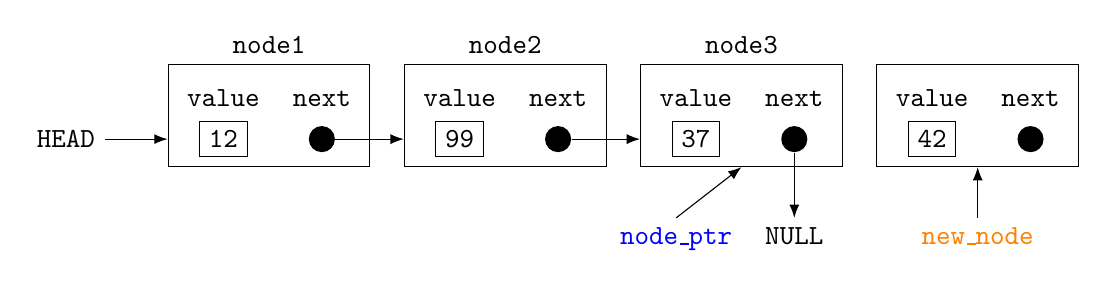
\begin{tikzpicture}
  \node[HEAD] at (-2,0) (HEAD) {HEAD};
  \pic at (0,0) {llnode=node1/12};
  \pic at (3,0) {llnode=node2/99};
  \pic at (6,0) {llnode=node3/37};

  \pic at (9,0) {llnodelabel=node4/42/};

  \draw[link] (node3 next) -- ++(0,-1) node (NULL_PTR) {};

  \node[NULL, below] at (NULL_PTR) (NULL) {NULL};

  \draw[link] (HEAD.east) -- (node1 next-|node1.west);
  \draw[link] (node1 next) -- (node1 next-|node2.west);
  \draw[link] (node2 next) -- (node2 next-|node3.west);
  % \draw[link] (node3 next) -- (NULL.west);

  \draw[link] (NULL_PTR) ++(-1.5,0) node (NODE_PTR) {} -- (node3.south);

  \node[PTR, below, text=blue] at (NODE_PTR) (NODE) {node\_ptr};

  \draw[arrows=Latex-] (node4.south) -- (NULL_PTR -| node4) node (node4 arrow) {};

  \node[PTR, below, text=orange] at (node4 arrow) () {new\_node};
\end{tikzpicture}

\end{document}
